\chapter{Quadrature Phase-Shift Keying (QPSK)}
\label{ch:qpsk}

\begin{nontechnical}
\textbf{QPSK is like using 4 different hand signals instead of 2}---you can send messages twice as fast!

\textbf{Simple idea:}
\begin{itemize}
\item Instead of just ``wave up'' or ``wave down'' (BPSK), QPSK uses \textbf{4 directions}
\item Up-right $\nearrow$ = 01 (bits)
\item Up-left $\nwarrow$ = 00
\item Down-left $\swarrow$ = 10
\item Down-right $\searrow$ = 11
\end{itemize}

\textbf{Real use:} Satellite TV (DVB-S) uses QPSK for reliable transmission from space. Your phone uses QPSK when cell signal is weak.

\textbf{Why 4 directions?} Sends 2 bits per symbol = twice as fast as BPSK! Still reliable because the 4 directions are well-separated.
\end{nontechnical}

\section{Overview}

\textbf{Quadrature Phase-Shift Keying (QPSK)} extends BPSK by using four phase states ($45°$, $135°$, $225°$, $315°$) to encode 2 bits per symbol, doubling spectral efficiency while maintaining robust performance.

\begin{keyconcept}
QPSK achieves \textbf{2 bits/symbol} (double that of BPSK) with \textbf{identical BER performance} at the same $E_b/N_0$, making it optimal for bandwidth-limited channels such as satellite downlinks and mobile communications.
\end{keyconcept}

QPSK is widely deployed in DVB-S satellite television, GPS modernized signals (L5), 4G LTE initial connection, and IEEE 802.11b WiFi.

\section{Mathematical Description}

\subsection{Time-Domain Signal}

The QPSK waveform is expressed as:
\begin{equation}
s(t) = A \cos(2\pi f_c t + \phi_n)
\end{equation}
where:
\begin{itemize}
\item $A$ = carrier amplitude (volts)
\item $f_c$ = carrier frequency (Hz)
\item $\phi_n \in \{45°, 135°, 225°, 315°\}$ = phase for symbol $n$
\end{itemize}

\textbf{Phase encoding (Gray mapping):}
\begin{equation}
\phi_n = \begin{cases}
45° & \text{if bits = 01} \\
135° & \text{if bits = 00} \\
225° & \text{if bits = 10} \\
315° & \text{if bits = 11}
\end{cases}
\end{equation}

\begin{calloutbox}{Gray Coding}
Adjacent constellation points differ by only 1 bit. This minimizes bit errors when noise causes a symbol to be decoded as an adjacent point (most common error). Example: $01$ ($45°$) adjacent to $00$ ($135°$)---differ by 1 bit only.
\end{calloutbox}

\subsection{IQ Representation}

The baseband complex representation is:
\begin{equation}
s(t) = I_n \cos(2\pi f_c t) - Q_n \sin(2\pi f_c t)
\end{equation}

\textbf{IQ components} for normalized symbols ($E_s = 1$):
\begin{equation}
I_n = A \cos(\phi_n), \quad Q_n = A \sin(\phi_n)
\end{equation}

For $A = \sqrt{2}$ (unit energy):

\begin{center}
\begin{tabular}{@{}ccccc@{}}
\toprule
Bits & Phase & $I_n$ & $Q_n$ & Complex \\
\midrule
01 & $45°$ & $+1$ & $+1$ & $1+j$ \\
00 & $135°$ & $-1$ & $+1$ & $-1+j$ \\
10 & $225°$ & $-1$ & $-1$ & $-1-j$ \\
11 & $315°$ & $+1$ & $-1$ & $1-j$ \\
\bottomrule
\end{tabular}
\end{center}

\textbf{Alternative representation:}
\begin{equation}
s(t) = \mathrm{Re}\{(I_n + jQ_n) e^{j2\pi f_c t}\}
\end{equation}

\section{Constellation Diagram}

The QPSK constellation consists of four points at the corners of a square, maximally separated for noise immunity:

\begin{center}
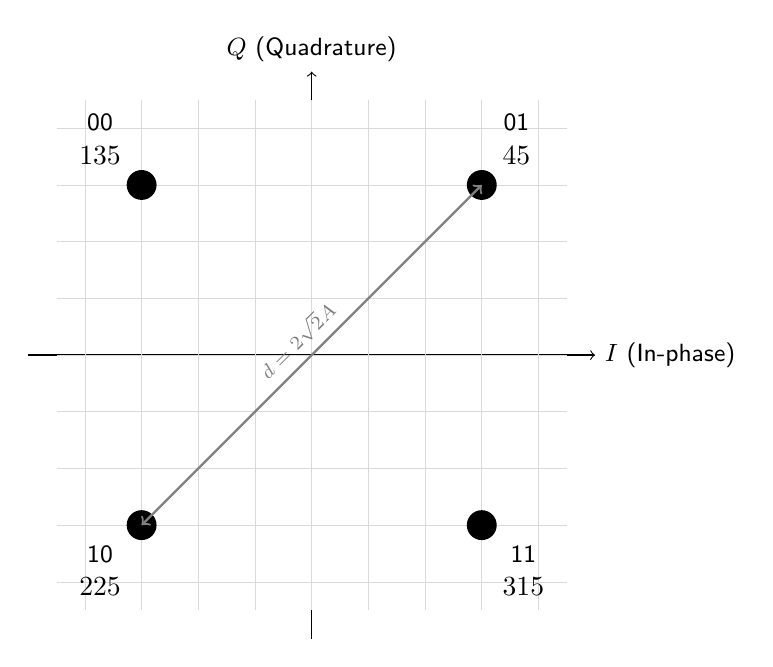
\begin{tikzpicture}[scale=1.8]
% Axes
\draw[->] (-2,0) -- (2,0) node[right] {\sffamily\small $I$ (In-phase)};
\draw[->] (0,-2) -- (0,2) node[above] {\sffamily\small $Q$ (Quadrature)};

% Grid
\draw[very thin,gray!30] (-1.8,-1.8) grid[step=0.4] (1.8,1.8);

% Constellation points
\fill[black] (1.2,1.2) circle (3pt);
\fill[black] (-1.2,1.2) circle (3pt);
\fill[black] (-1.2,-1.2) circle (3pt);
\fill[black] (1.2,-1.2) circle (3pt);

% Labels
\node[above right=4pt,align=center] at (1.2,1.2) {\sffamily\small 01\\$45°$};
\node[above left=4pt,align=center] at (-1.2,1.2) {\sffamily\small 00\\$135°$};
\node[below left=4pt,align=center] at (-1.2,-1.2) {\sffamily\small 10\\$225°$};
\node[below right=4pt,align=center] at (1.2,-1.2) {\sffamily\small 11\\$315°$};

% Distance annotation
\draw[<->,thick,gray] (1.2,1.2) -- (-1.2,-1.2) node[midway,above,sloped] {\sffamily\scriptsize $d = 2\sqrt{2}A$};
\end{tikzpicture}
\end{center}

The minimum Euclidean distance between any two symbols is $d = 2A$, identical to BPSK at the same power, ensuring equivalent BER performance.

\section{Modulation and Demodulation}

\subsection{Transmitter (QPSK Modulator)}

\begin{center}
\begin{tikzpicture}[
  block/.style={rectangle, draw, minimum width=2cm, minimum height=1cm, font=\sffamily\small, align=center},
  node distance=2cm,
  font=\small
]
\node[align=center] (input) {\sffamily Binary\\$\{b_0, b_1\}$};
\node[block, right of=input, node distance=2.5cm] (demux) {Serial-to-\\Parallel};
\node[block, above right of=demux, node distance=3cm] (map_i) {Map to\\$I_n$};
\node[block, below right of=demux, node distance=3cm] (map_q) {Map to\\$Q_n$};
\node[block, right of=map_i, node distance=3cm] (mult_i) {Mixer\\$\times$};
\node[block, right of=map_q, node distance=3cm] (mult_q) {Mixer\\$\times$};
\node[above of=mult_i, node distance=1.3cm, font=\scriptsize] (carrier_i) {$\cos(2\pi f_c t)$};
\node[below of=mult_q, node distance=1.3cm, font=\scriptsize] (carrier_q) {$-\sin(2\pi f_c t)$};
\node[draw,circle,right of=mult_i, node distance=2.5cm,yshift=-1.5cm] (sum) {$+$};
\node[block, right of=sum, node distance=2.5cm] (filter) {Bandpass\\Filter};
\node[align=center, right of=filter, node distance=2.5cm] (output) {\sffamily QPSK\\Output};

\draw[->,thick] (input) -- (demux);
\draw[->,thick] (demux) -| node[near end,above,font=\scriptsize] {$b_0$} (map_i);
\draw[->,thick] (demux) -| node[near end,below,font=\scriptsize] {$b_1$} (map_q);
\draw[->,thick] (map_i) -- node[above,font=\scriptsize] {$I_n$} (mult_i);
\draw[->,thick] (map_q) -- node[above,font=\scriptsize] {$Q_n$} (mult_q);
\draw[->,thick] (carrier_i) -- (mult_i);
\draw[->,thick] (carrier_q) -- (mult_q);
\draw[->,thick] (mult_i) -| (sum);
\draw[->,thick] (mult_q) -| (sum);
\draw[->,thick] (sum) -- (filter);
\draw[->,thick] (filter) -- (output);
\end{tikzpicture}
\end{center}

\textbf{Modulation process:}
\begin{enumerate}
\item \textbf{Serial-to-parallel conversion:} Split incoming bit stream into 2-bit pairs
\item \textbf{Bit mapping:} Convert bits to IQ values ($\pm 1$)
\item \textbf{I-channel:} Multiply $I_n$ by carrier: $I_n \cos(2\pi f_c t)$
\item \textbf{Q-channel:} Multiply $Q_n$ by $90°$ shifted carrier: $-Q_n \sin(2\pi f_c t)$
\item \textbf{Combine:} Add I and Q components
\item \textbf{Pulse shaping:} Apply raised-cosine filter to limit bandwidth
\end{enumerate}

\begin{keyconcept}
QPSK = \textbf{Two independent BPSK channels} (I and Q) operating simultaneously at $90°$ phase separation. This orthogonality allows both channels to coexist without interference.
\end{keyconcept}

\subsection{Receiver (Coherent Detector)}

\begin{center}
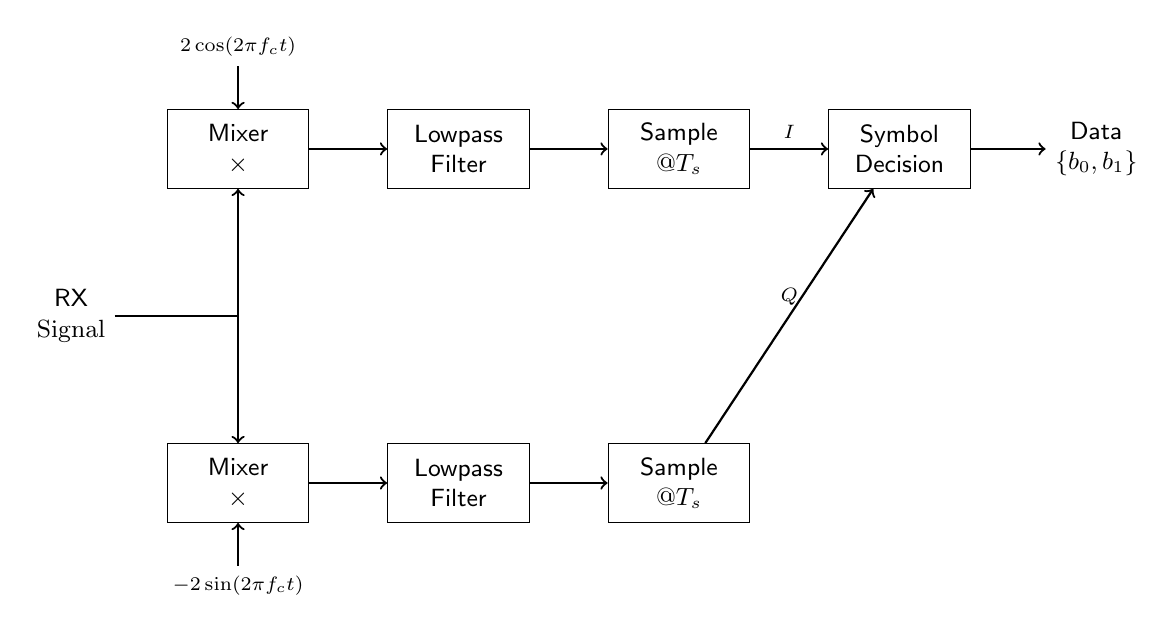
\begin{tikzpicture}[
  block/.style={rectangle, draw, minimum width=1.8cm, minimum height=1cm, font=\sffamily\small, align=center},
  node distance=2cm,
  font=\small
]
\node[align=center] (input) {\sffamily RX\\Signal};
\node[block, above right of=input, node distance=3cm] (mult_i) {Mixer\\$\times$};
\node[block, below right of=input, node distance=3cm] (mult_q) {Mixer\\$\times$};
\node[above of=mult_i, node distance=1.3cm, font=\scriptsize, align=center] (lo_i) {$2\cos(2\pi f_c t)$};
\node[below of=mult_q, node distance=1.3cm, font=\scriptsize, align=center] (lo_q) {$-2\sin(2\pi f_c t)$};
\node[block, right of=mult_i, node distance=2.8cm] (lpf_i) {Lowpass\\Filter};
\node[block, right of=mult_q, node distance=2.8cm] (lpf_q) {Lowpass\\Filter};
\node[block, right of=lpf_i, node distance=2.8cm] (sample_i) {Sample\\$@T_s$};
\node[block, right of=lpf_q, node distance=2.8cm] (sample_q) {Sample\\$@T_s$};
\node[block, right of=sample_i, node distance=2.8cm] (decide) {Symbol\\Decision};
\node[align=center, right of=decide, node distance=2.5cm] (output) {\sffamily Data\\$\{b_0,b_1\}$};

\draw[->,thick] (input) -| (mult_i);
\draw[->,thick] (input) -| (mult_q);
\draw[->,thick] (lo_i) -- (mult_i);
\draw[->,thick] (lo_q) -- (mult_q);
\draw[->,thick] (mult_i) -- (lpf_i);
\draw[->,thick] (mult_q) -- (lpf_q);
\draw[->,thick] (lpf_i) -- (sample_i);
\draw[->,thick] (lpf_q) -- (sample_q);
\draw[->,thick] (sample_i) -- node[above,font=\scriptsize] {$I$} (decide);
\draw[->,thick] (sample_q) -- node[above,font=\scriptsize] {$Q$} (decide);
\draw[->,thick] (decide) -- (output);
\end{tikzpicture}
\end{center}

\textbf{Demodulation process:}
\begin{enumerate}
\item \textbf{I-channel:} Multiply by $2\cos(2\pi f_c t)$, lowpass filter $\rightarrow$ recovers $I_n$
\item \textbf{Q-channel:} Multiply by $-2\sin(2\pi f_c t)$, lowpass filter $\rightarrow$ recovers $Q_n$
\item \textbf{Sample:} At symbol period $T_s$: $(I_n, Q_n)$
\item \textbf{Decision:} Find nearest constellation point based on received $(I, Q)$
  \begin{itemize}
  \item If $I > 0$ and $Q > 0$ $\rightarrow$ bits = 01
  \item If $I < 0$ and $Q > 0$ $\rightarrow$ bits = 00
  \item If $I < 0$ and $Q < 0$ $\rightarrow$ bits = 10
  \item If $I > 0$ and $Q < 0$ $\rightarrow$ bits = 11
  \end{itemize}
\end{enumerate}

\begin{warningbox}
\textbf{Carrier synchronization is critical.} Both frequency and phase must match the transmitter. A phase offset $\phi_e$ rotates the entire constellation, causing symbol errors. Advanced techniques like Costas loop or decision-directed feedback are required.
\end{warningbox}

\section{Bit Error Rate (BER) Performance}

\subsection{QPSK in AWGN Channel}

For ideal coherent detection:
\begin{equation}
\mathrm{BER}_{\mathrm{QPSK}} = Q\left(\sqrt{\frac{2E_b}{N_0}}\right) = \frac{1}{2}\mathrm{erfc}\left(\sqrt{\frac{E_b}{N_0}}\right)
\end{equation}
where:
\begin{itemize}
\item $E_b = \frac{E_s}{2}$ = energy per bit (joules)
\item $E_s = A^2 T_s$ = energy per symbol (joules)
\item $N_0$ = noise power spectral density (W/Hz)
\item $Q(x) = \frac{1}{\sqrt{2\pi}}\int_x^\infty e^{-t^2/2}\,dt$ (Gaussian Q-function)
\end{itemize}

\textbf{Key insight:} QPSK has identical BER to BPSK at the same $E_b/N_0$ because symbol energy $E_s = 2E_b$ for QPSK (2 bits/symbol).

\textbf{Performance benchmarks:}

\begin{center}
\begin{tabular}{@{}lrl@{}}
\toprule
$E_b/N_0$ (dB) & \multicolumn{1}{c}{BER} & Spectral Efficiency \\
\midrule
6~dB & $5.0 \times 10^{-3}$ & 2~bps/Hz \\
8~dB & $4.0 \times 10^{-4}$ & 2~bps/Hz \\
10~dB & $3.9 \times 10^{-6}$ & 2~bps/Hz \\
12~dB & $1.3 \times 10^{-8}$ & 2~bps/Hz \\
\bottomrule
\end{tabular}
\end{center}

\subsection{Symbol Error Rate (SER)}

The probability of symbol error (2-bit error or 1-bit error) is higher than BER:
\begin{equation}
\mathrm{SER}_{\mathrm{QPSK}} \approx 2Q\left(\sqrt{\frac{2E_b}{N_0}}\right)
\end{equation}

With Gray coding, most symbol errors affect only 1 bit, so:
\begin{equation}
\mathrm{BER} \approx \frac{\mathrm{SER}}{2}
\end{equation}

\section{Bandwidth Efficiency}

The symbol rate for QPSK is:
\begin{equation}
R_s = \frac{R_b}{2}
\end{equation}
where $R_b$ is the bit rate (bps) and $R_s$ is the symbol rate (symbols/s).

With raised-cosine pulse shaping (roll-off $\alpha$):
\begin{equation}
B = R_s(1 + \alpha) = \frac{R_b}{2}(1 + \alpha)
\end{equation}

\textbf{Spectral efficiency:}
\begin{equation}
\eta = \frac{R_b}{B} = \frac{2}{1+\alpha}
\end{equation}

For $\alpha = 0.35$: $\eta \approx 1.48$~bps/Hz (double that of BPSK).

\begin{calloutbox}{Example: 2~Mbps QPSK System}
\begin{itemize}
\item Data rate: $R_b = 2$~Mbps
\item Symbol rate: $R_s = 1$~Msps
\item Roll-off: $\alpha = 0.35$
\item Required bandwidth: $B = 1 \times (1 + 0.35) = 1.35$~MHz
\item Spectral efficiency: $\eta = 2/1.35 = 1.48$~bps/Hz
\end{itemize}

\textbf{QPSK transmits the same data rate as BPSK using half the bandwidth.}
\end{calloutbox}

\section{Worked Example: DVB-S Satellite Link}

\textbf{Scenario:} DVB-S QPSK downlink from geostationary satellite

\subsection*{Given Parameters}

\begin{tabular}{@{}ll@{}}
TX power & $P_t = 50$~W = 47~dBm \\
TX antenna gain & $G_t = 32$~dBi \\
Distance & $d = 38{,}500$~km (GEO orbit) \\
Frequency & $f = 11.5$~GHz (Ku-band) \\
RX antenna gain & $G_r = 33$~dBi (60~cm dish) \\
System noise temp & $T_s = 125$~K \\
Symbol rate & $R_s = 20$~Msps \\
Required BER & $10^{-6}$ (before FEC) \\
\end{tabular}

\subsection*{Step 1: Free-Space Path Loss}

\begin{equation}
\mathrm{FSPL\,[dB]} = 20\log_{10}(d_{\text{km}}) + 20\log_{10}(f_{\text{MHz}}) + 32.45
\end{equation}
\begin{equation}
\mathrm{FSPL} = 20\log_{10}(38{,}500) + 20\log_{10}(11{,}500) + 32.45 = 205.8~\text{dB}
\end{equation}

\subsection*{Step 2: Received Signal Power}

\begin{equation}
P_r = P_t + G_t + G_r - \mathrm{FSPL} = 47 + 32 + 33 - 205.8 = -93.8~\text{dBm}
\end{equation}

\subsection*{Step 3: Noise Power}

Bandwidth $B = R_s(1 + \alpha) = 20 \times 1.35 = 27$~MHz

\begin{equation}
N = kT_sB = (1.38 \times 10^{-23})(125)(27 \times 10^6) = 4.66 \times 10^{-14}~\text{W}
\end{equation}
\begin{equation}
N = 10\log_{10}(4.66 \times 10^{-14} / 10^{-3}) = -103.3~\text{dBm}
\end{equation}

\subsection*{Step 4: $E_b/N_0$ Calculation}

\begin{equation}
C/N = P_r - N = -93.8 - (-103.3) = 9.5~\text{dB}
\end{equation}

For QPSK (2 bits/symbol):
\begin{equation}
\frac{E_b}{N_0} = \frac{C}{N} + 10\log_{10}\left(\frac{B}{R_b}\right) = 9.5 + 10\log_{10}\left(\frac{27}{40}\right) = 9.5 + (-1.7) = 7.8~\text{dB}
\end{equation}

\subsection*{Step 5: Link Assessment}

\begin{itemize}
\item \textbf{Required $E_b/N_0$ for BER $= 10^{-6}$:} 10.5~dB
\item \textbf{Available $E_b/N_0$:} 7.8~dB
\item \textbf{Shortfall:} $-2.7$~dB
\end{itemize}

\begin{calloutbox}[colback=black!8!white,colframe=black]{Link Budget Conclusion}
\textbf{Result: Link does NOT close without Forward Error Correction (FEC)}

DVB-S standard employs:
\begin{itemize}
\item Convolutional coding (rate 1/2, 2/3, 3/4, 5/6, 7/8)
\item Reed-Solomon outer code (204,188)
\item Typical coding gain: 4--6~dB
\end{itemize}

With rate 3/4 FEC (coding gain $\sim$4.5~dB): Effective $E_b/N_0 = 7.8 + 4.5 = 12.3$~dB

\textbf{Final margin:} $12.3 - 10.5 = 1.8$~dB (acceptable for clear-sky conditions)
\end{calloutbox}

\section{Practical Applications}

\subsection{DVB-S/DVB-S2 Satellite Television}

\textbf{Usage:} European satellite TV standard for broadcasting
\begin{itemize}
\item \textbf{Modulation:} QPSK (DVB-S), QPSK/8PSK/16APSK (DVB-S2)
\item \textbf{Frequency:} 10.7--12.75~GHz (Ku-band)
\item \textbf{Symbol rate:} 20--30~Msps typical
\item \textbf{FEC:} Concatenated (Convolutional + Reed-Solomon)
\item \textbf{Rationale:} Robust against rain fade and satellite power limitations
\end{itemize}

\subsection{GPS Modernized Signals (L5)}

\textbf{Usage:} Improved civilian GPS signal
\begin{itemize}
\item \textbf{Frequency:} 1176.45~MHz (L5 band)
\item \textbf{Modulation:} QPSK with DSSS
\item \textbf{Chip rate:} 10.23~Mcps
\item \textbf{Data rate:} 100~bps (navigation message)
\item \textbf{Advantage:} 2× power efficiency vs BPSK for dual civil codes (I and Q)
\end{itemize}

\subsection{4G LTE Initial Access}

\textbf{Usage:} Mobile broadband connection establishment
\begin{itemize}
\item \textbf{Channel:} Physical Downlink Control Channel (PDCCH)
\item \textbf{Modulation:} QPSK for initial sync, control, low SNR users
\item \textbf{Adaptive:} Switches to 16-QAM, 64-QAM, 256-QAM at higher SNR
\item \textbf{Rationale:} QPSK ensures reliable connection at cell edge
\end{itemize}

\subsection{IEEE 802.11b WiFi}

\textbf{Usage:} Legacy 2.4~GHz WiFi
\begin{itemize}
\item \textbf{Modulation:} QPSK with DSSS/CCK
\item \textbf{Data rate:} 2~Mbps (QPSK), 5.5/11~Mbps (CCK)
\item \textbf{Frequency:} 2.4~GHz ISM band
\item \textbf{Legacy:} Replaced by OFDM in 802.11a/g/n/ac/ax
\end{itemize}

\section{Advantages and Disadvantages}

\subsection*{Advantages}

\begin{enumerate}
\item \textbf{Double spectral efficiency:} 2~bps/Hz vs 1~bps/Hz for BPSK
\item \textbf{Same BER as BPSK:} Identical $E_b/N_0$ requirement for given BER
\item \textbf{Constant envelope:} Compatible with nonlinear amplifiers
\item \textbf{Widely standardized:} Mature technology with extensive ecosystem
\item \textbf{Simple implementation:} Two independent BPSK channels (I and Q)
\end{enumerate}

\subsection*{Disadvantages}

\begin{enumerate}
\item \textbf{Carrier synchronization complex:} Requires accurate frequency and phase recovery
\item \textbf{Quadrature errors:} IQ imbalance degrades performance
\item \textbf{Lower efficiency than QAM:} 16-QAM, 64-QAM offer higher throughput at good SNR
\item \textbf{Phase ambiguity:} $90°$ rotational ambiguity requires differential encoding or preamble
\item \textbf{Symbol timing critical:} Requires precise clock recovery
\end{enumerate}

\section{Summary}

\begin{center}
\begin{tabular}{@{}ll@{}}
\toprule
\textbf{Parameter} & \textbf{Value} \\
\midrule
Bits per symbol & 2 \\
Constellation points & 4 ($45°$, $135°$, $225°$, $315°$) \\
Spectral efficiency & $\sim$1.5--2.0~bps/Hz \\
BER @ 10~dB $E_b/N_0$ & $3.9 \times 10^{-6}$ \\
Bandwidth vs BPSK & 50\% (half) \\
Carrier recovery & Required (Costas loop) \\
Implementation & Moderate complexity \\
Best application & Bandwidth-limited channels \\
Typical uses & Satellite, GPS, LTE, WiFi \\
\bottomrule
\end{tabular}
\end{center}

\section{Further Reading}

\begin{itemize}
\item \textbf{Chapter~\ref{ch:bpsk}:} Binary Phase-Shift Keying---foundation of QPSK
\item \textbf{Chapter 8:} 8PSK \& Higher-Order PSK---extension to 3+ bits/symbol
\item \textbf{Chapter 9:} Quadrature Amplitude Modulation (QAM)---higher efficiency
\item \textbf{Chapter 12:} Constellation Diagrams---visualization techniques
\item \textbf{Chapter 13:} IQ Representation---complex baseband mathematics
\item \textbf{Chapter 18:} Bit Error Rate Analysis---performance measurement
\item \textbf{Chapter 22:} Forward Error Correction---coding for BER improvement
\item \textbf{Chapter 25:} Carrier Recovery Techniques---synchronization methods
\end{itemize}
